\section{Metody XAI} \label{metody_xai}
Interpretowalność możemy podzielić ze względu na sposób jej przeprowadzenia. Modele proste strukturalnie i w zrozumieniu, niewymagające przy tym od nas żadnych zewnętrznych pomocy są określane mianem interpretowalnych przez design. Post-hoc odnosi się do~trudniejszych systemów, na których dopiero po przeprowadzeniu uczenia stosujemy metody XAI. Dzieli się to na dwa podejścia - niezależne i zależne od modelu. Z tych pierwszych dodatkowo rozróżniamy lokalne - tłumaczące wskazane przypadki oraz globalne - analizujące dane wejściowe \cite{molnar2025}.

\subsection{LIME}
LIME \cite{molnar2025, oreilly_lime}, jak mówi też rozszerzenie jego skrótu (ang. \textit{Local interpretable model-agnostic explanations}), jest lokalnie interpretowanymi wyjaśnieniami niezależnymi do modelu, czyli należy do grupy post-hoc. Został on zaprojektowany przez Ribeiro, Singha i Guestrina – specjalistów w dziedzinie AI. Jego działanie zostało zaprezentowane na Rys. \ref{fig:lime_picture}. Metoda polega na zaburzeniu danych wejściowych w celu stworzenia nowego zbioru, który jest następnie poddawany ocenie poprzez diagnozowany model sztucznej inteligencji, będący czarną skrzynką. Przypisuje on temu nowo powstałemu zbiorowi wartości przewidywane. Następnie na tych danych uczony jest interpretowalny model (jeden z prostszych systemów, np. drzewo decyzyjne), który jest oceniany na podstawie podobieństwa próbkowanych instancji do tych, z których dane próby powstały. Powstał wzór obrazujący to porównanie:

\begin{equation} \label{lime_eqn}
explanation(x)\ =\ arg\ min_{g\ \in\ G}\ L(f,\ g,\ \pi_x)\ +\ \Omega(g)
\end{equation}

gdzie: wyjaśnienie dla badanej próbki oznaczonej jako $x$, to model $g$ minimalizujący funkcję straty, tutaj $L$, która mierzy jak blisko jest owa predykcja do predykcji modelu oryginalnego $f$, biorąc pod uwagę sąsiedztwo próbki $x$, którego używamy do wyjaśnienia - $\pi_x$. Dodatkowo obecna jest zmienna $\Omega(g)$ mówiąca o złożoności modelu, określanej jako ilość zmiennych. Dziedzina $G$ opisuje przestrzeń wszystkich możliwych modeli interpretowalnych danego typu. 
	
Wyjaśnienie predykcji odbywa się za pomocą interpretacji modelu lokalnego (powstałego wskutek metody LIME). To rozwiązanie daje dobre dopasowania lokalne, jednak nie gwarantuje poprawnych wyników globalnie (tzw. \textit{local fidelity}). Problematyczne może być wybranie odpowiedniego modelu surrogacyjnego oraz wielkości sąsiedztwa branego pod uwagę podczas analizy próbki. Zbyt duży obszar powoduje wpływ mało istotnych elementów (leżących daleko od badanej próby) na wynik przewidywań, a za małe to, że skupiamy się na~tym, co leży najbliżej, skutkując w możliwości pominięcia innych istotnych czynników.

Za pomocą LIME można analizować obrazy, dane tekstowe czy tabelaryczne. W przypadku zdjęć, zaburzenie danych odbywa się poprzez włączenie lub wyłączenie zbiorów pikseli dobieranych w grupy na podstawie sąsiedztwa oraz koloru. W celu przerobienia danych przechowywanych w tabelach, metoda zmienia każdą z cech (wartości z kolumn) oddzielnie, kierując się rozkładem normalnym ze średnią i odchyleniem standardowym obliczonymi dla danej cechy.

 \begin{figure}[H]
     \centering
     
\includegraphics[width=0.9\linewidth]{lime.jpg}
     \caption{Sposób działaia metody LIME \cite{lime_picture_medium}}
     \label{fig:lime_picture}
 \end{figure}

Jedną z największych wad omawianej metody, oprócz problemu z doborem wielkości branego pod uwagę sąsiedztwa próby, jest brak stabilności w wynikach predykcji. Jeśli ponownie przeprowadzimy podział danych, to może się zdarzyć, że LIME poda inne wyjaśnienia pomimo dużej zbieżności próbek do tych, pochodzących z poprzedniej selekcji. Kolejnym problemem jest możliwość powstania danych, które nie mają odwzorowania w~świecie rzeczywistym bądź są skrajnie rzadkie. Takie przypadki powstają podczas tworzenia nowych zaburzonych informacji z tych już istniejących. Niemniej jednak metoda jest prosta w implementacji i zrozumieniu oraz generuje przejrzyste wyniki. Poprzez umiejętność analizowania różnych typów zmiennych, może być wszechstronnie używana. Dodatkowo zbiory przedstawione modelowi oryginalnemu, a LIME, nie muszą być jednakowe. Często, ze względu na~olbrzymi format danych używa się specjalnych metod, mających na celu zmniejszenie ich wymiarów lub stosuje się normalizację. Taka transformacja sprawia, że przybierają one nie dającą się pojąć dla ludzi formę. Dzięki zastosowaniu w owej metodzie pierwotnych zbiorów zachowujemy ich czytelniejszą strukturę.  

Przykładowy wykres słupkowy, zaprezentowany na Rys. \ref{fig:lime_barchar_example}, przedstawia średnie wagi LIME cech poszczególnych klas obliczone z ich wartości bezwzględnych. Wagi zostały uzyskane ze wszystkich próbek zbioru treningowego. Wykres nie prezentuje, jaki rodzaj wpływu miała przedstawiona cecha, czyli to, czy zwiększała bądź zmniejszała predykcję, a jedynie jej natężenie wpływu - to jak duże lub małe miała znaczenie na predykcję. Legenda umieszczona w prawym górnym rogu pokazuje jaki kolor odpowiada danej klasie. Wartościami osi OX są cechy, a OY średnie wagi LIME. Jest on w pracy wykorzystywany jedynie w problemie klasyfikacji wieloklasowej.

\begin{figure}[H]
    \centering
    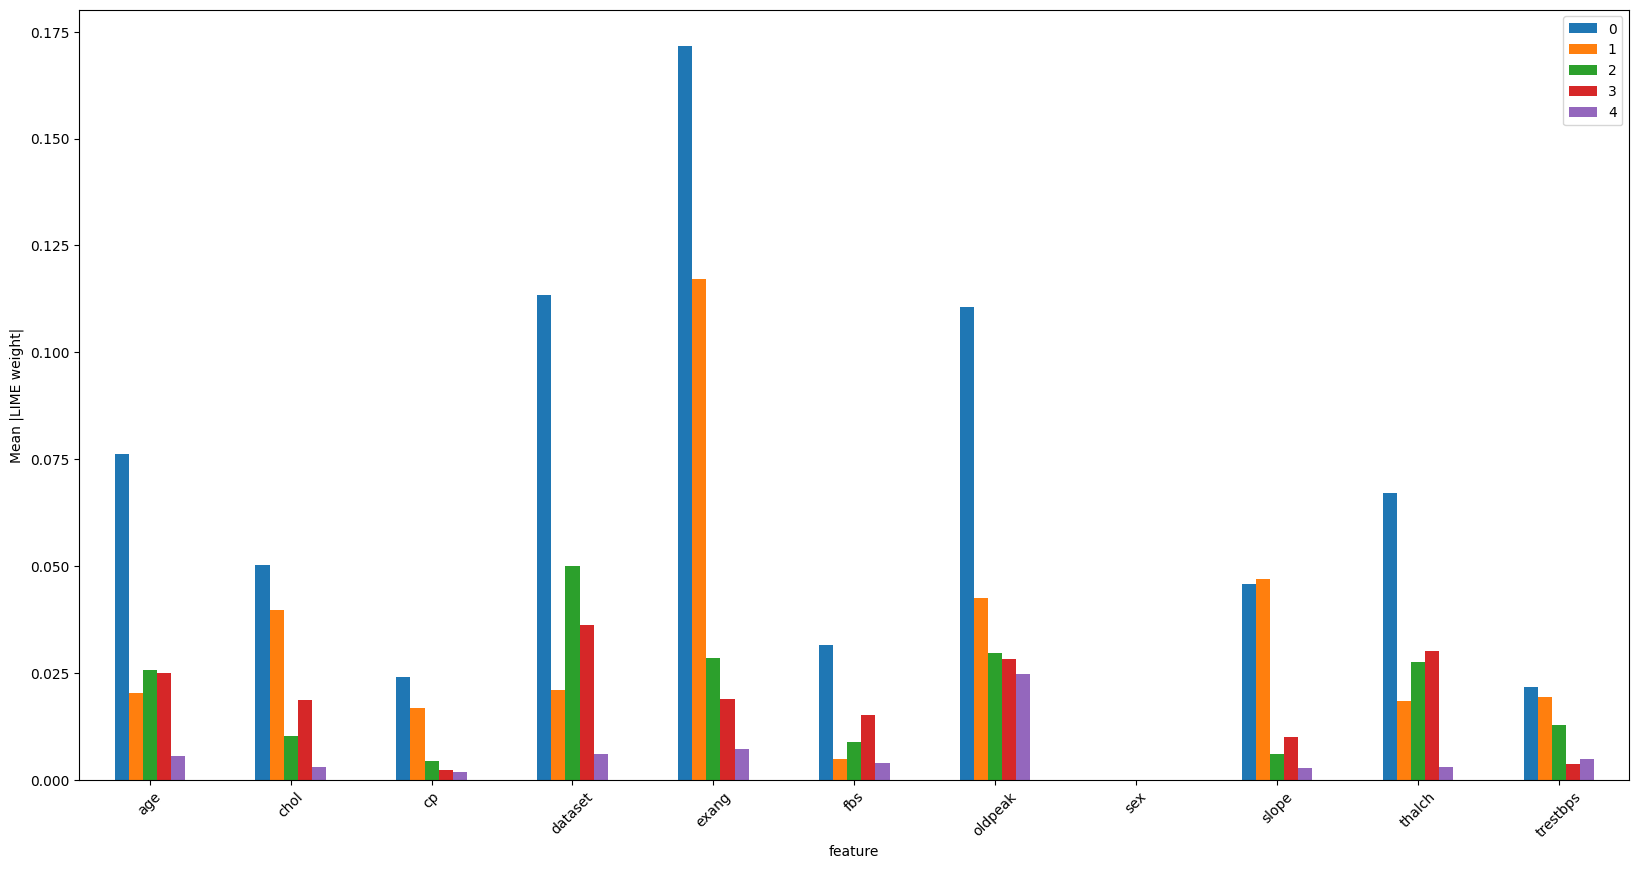
\includegraphics[width=0.85\linewidth]{rysunki/heart/lime_barchar_rf_heart.png}
    \caption{Przykładowy wykres słupkowy średnich wartości bezwzględnych wag LIME dla każdej z klasy  [źródło własne]}
    \label{fig:lime_barchar_example}
\end{figure}

Drugim używanym w pracy wykresem, przedstawiającym tłumaczenie metody LIME dla danych tabelarycznych, jest ten, przedstawiony na Rys. \ref{fig:lime_absolutemeanplot_example}. To połączenie zebranych wcześniej średnich wartości bezwzględnych wag LIME dla poszczególnych klas. Wyniki, uzyskane dla każdej z klasy, zostały złączone za pomocą średniej arytmetycznej w jedną liczbę określającą ogólną istotność cechy. Z racji, że dane są obliczane na podstawie wartości bezwzględnych, nie prezentuje on jaki rodzaj wpływu miała każda z cech. Oś OX prezentuje średnie wagi LIME, a OY cechy.

\begin{figure}[H]
    \centering
    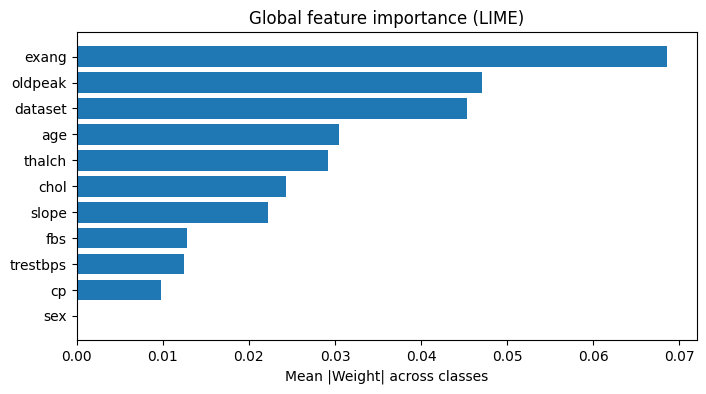
\includegraphics[width=0.70\linewidth]{rysunki/heart/lime_absolutemeanplot_rf_heart.png}
    \caption{Przykładowy wykres średnich obliczonych z bezwzględnych wartości wag LIME [źródło własne]}
    \label{fig:lime_absolutemeanplot_example}
\end{figure}

Na Rys. \ref{fig:lime_image_example} zostało zamieszczone przykładowe tłumaczenie próbki, w postaci obrazu, uzyskane za pomocą metody LIME. Pierwsze zdjęcie, nad którym widnieje napis ,,hide\_rest=True'', przedstawia jedynie 5 najbardziej wpływowych obszarów wskazanych przez LIME. Reszta obrazu wejściowego została wyłączona. Środkowa część, zatytułowana ,,hide\_rest=False'', również prezentuje 5 najistotniejszych fragmentów, ale z resztą analizowanego zdjęcia. Ostatnia wizualizacja, opisana jako ,,Influence'', pokazuje 10 elementów uznanych przez metodę jako najważniejsze w przewidywaniu. Kolorem zielonym zostały oznaczone te, które mają przemawiają za wskazaną przez model predykcją, a czerwonym - jej przeciwne. 

\begin{figure}[H]
    \centering
    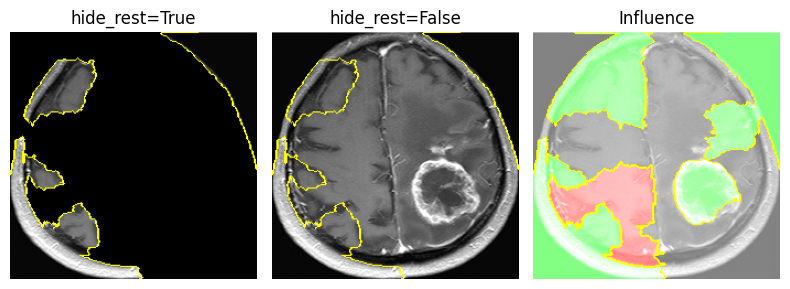
\includegraphics[width=0.75\linewidth]{rysunki/brain/lime_vgg16_1_brain.png}
    \caption{Przykładowe wyniki uzyskane po zbadaniu próbki za pomocą metody LIME [źródło własne]}
    \label{fig:lime_image_example}
\end{figure}


\subsection{SHAP}
SHAP (ang. SHapley Additive exPlanations) \cite{molnar2025, ALI2023101805, shap_explanation_yt} jest kolejną niezależną lokalną metodą post-hoc, za pomocą której możemy analizować dane tekstowe, tabelaryczne i obrazy. Bazuje ona na wartościach Shapley’a z teorii gier. Polega to, na tym, że każdą z~cech (lub grupy cech, np. grupę pikseli) określamy mianem gracza grającego w grę (naukę modelu), gdzie nagrodą jest przewidywanie modelu, którą musimy rozdzielić pomiędzy graczy w zależności od ich wkładu w jej zdobycie (wpływ na wynik). Odpowiedzią powinny być wartości mówiące, jakie zaangażowanie miała każda ze zmiennych użyta do konkretnej predykcji w porównywaniu ze średnią prognozą, czyli wyjaśnienie, czemu przypadek odbiega od wartości przeciętnej. Może to przypominać regresję liniową, jednak nie potrafi ona wychwytywać zależności pomiędzy graczami (cechami), zwanych korelacjami, co czyni ją niezadowalającym rozwiązaniem. 

Do obliczenia wartości Shapley'a cechy, brane są pod uwagę jej istniejące związki z innymi czynnikami. W praktyce, zakładając sytuację zaprezentowaną na Rys. \ref{fig:shap_picture}, gdzie rozważamy wszystkie możliwe do stworzenia korelacje 3 elementowego zbioru, w którym wszystkie cechy są ze sobą powiązane, oznaczałoby to łącznie 8 różnych możliwości - brak koalicji, 3 wartości bazowe, 3 koalicje dwu-argumentowe i 1 koalicję trzy-argumentową. Następnie dla każdej możliwej kolejności dołączania graczy wyznacza się wkład poszczególnych cech do wartości pełnej koalicji. Średnia z uzyskanych w ten sposób wkładów jest wartością Shapley'a. Jak można zauważyć ilość przeprowadzanych działań rośnie wykładniczo wraz z wielkością zbioru cech. W celu rozwiązania tego problemu możemy skupić się tylko na wybranych związkach, co skutkuje uzyskaniem przybliżenia dokładnej wartości. Jeśli, jakaś zmienna jest niezależna od badanej, jej wartości są dobierane losowo (albo zamieniane na inne dostępne o ile badane dane są tabelaryczne). SHAP wyróżnia się tym, że~dodaje wpływy cech. Wyjaśnienie określone jest zależnością:

\begin{equation} \label{shap_eqn}
g(z')\ =\ \phi_0\ +\ \sum_{j=1}^{M} \phi_j\ z'_j
\end{equation}

gdzie, $g$ jest modelem objaśniającym, $z' = (z'_1,\dots, z'_M)^T \in\{0,1\}^M$ jest wskaźnikiem mówiącym czy dana zmienna występuje w równaniu (przyjmuje wartość 0 jeśli jej nie ma, 1 jeśli jest obecna), $M$ to maksymalna wielkość koalicji, a $\phi_j \in \mathbb{R}$ oznacza wartość Shapley'a cechy $j$. Wartość Shapley'a przedstawiona jest wzorem:

\begin{equation} \label{shap_eqn2}
\phi_j\ =\ \sum_{S\subseteq\{1,...,p\}\{i\}} \frac{|S|!(p-|S|-1)!}{p!}\left[val(S\ \cup\ \{i\})\ -\ val(S)\right] 
\end{equation}

w którym wartości oznaczają: $\sum_{S\subseteq\{1,...,p\}\{i\}}$ sumę wszystkich koalicji, do których gracz $i$ może dołączyć, $p!$ - ilość możliwych do stworzenia koalicji z $p$ graczy, $S$ - ilość graczy w~danej koalicji, $|S|!$ - ilość możliwości z jakich może powstać koalicja $S$, $(p-|S|-1)!$ - ilość możliwości dołączenia do koalicji przez innych graczy po tym jak gracz $i$ do niej dołączył, $val(S\ \cup\ \{i\})$ - wartość koalicji zawierającej gracza $i$, $val(S)$ - wartość koalicji, w~której nie ma gracza $i$.

\begin{figure}[H]
    \centering
    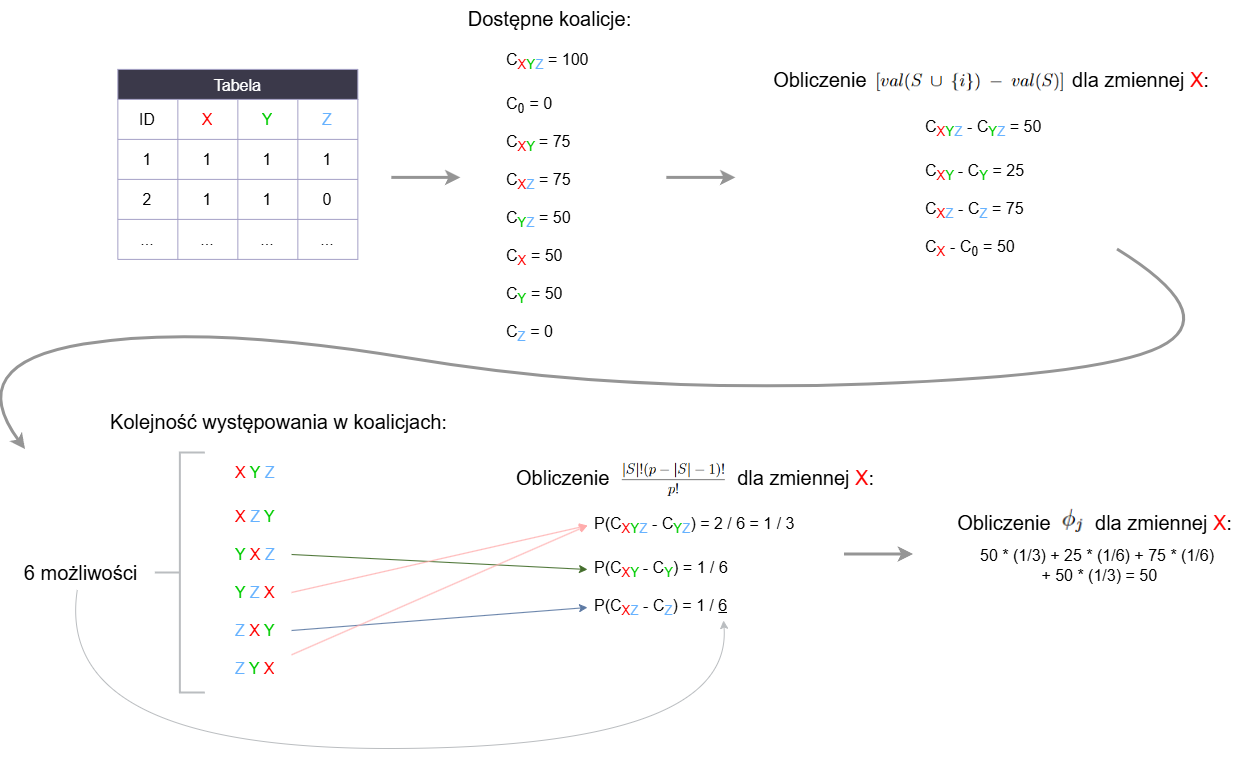
\includegraphics[width=1\linewidth]{rysunki/shap_drawio.png}
    \caption{Sposób działania metody SHAP [źródło własne]}
    \label{fig:shap_picture}
\end{figure}

Przy interpretacji wartości Shapley’a należy zachować ostrożność. Intuicyjnie wartości te, mogłyby być interpretowane jako różnica w przewidywaniu po usunięciu cechy. Jest to błędne podejście, ponieważ nie pełnią one takiej roli – mówią tylko o wpływie cechy na~prognozę w różnych koalicjach, a nie, co się stanie przy jej nieobecności. SHAP łączy w sobie LIME oraz wartości Shapley’a. Zyskuje dzięki temu podstawy pochodzące z teorii gier – równomierny rozkład wkładu w wynik końcowy pomiędzy cechami oraz kontrastowe wyjaśnienia. Niestety, cierpi on na długi czas wykonywania obliczeń spowodowany ilością różnych możliwych koalicji. Początkowo stosowanym sposobem obliczania wartości Shapley’a był KernelSHAP, który wykonywał obliczenia dla wszystkich znanych koalicji. W~celu uporania się z problemem złożoności obliczeniowej, powstały dwie alternatywy. TreeSHAP jest skoncentrowany na modelach drzewiastych, czyli np. lasach losowych, podczas gdy druga możliwość polega na permutacji w przód i wstecz, dzięki czemu uzyskujemy dwa obliczenia za~jedną koalicję. SHAP posiada też inną bardzo istotną wadę – jeśli model jest uprzedzony, co do pewnych klas decyzyjnych, metoda może tworzyć niepozornie wyglądające wyjaśnienia, niepokazujące jego nierównego traktowania. W przypadku modelu XGBoost SHAP w zadaniach klasyfikacji zwraca tzw. \textit{log odds}, a nie prawdopodobieństwo predykcji. Oznaczają one logarytm szansy, czyli logarytm z prawdopodobieństwa zaklasyfikowania jako dana klasa dzielone przez prawdopodobieństwo przeciwne \cite{gfg_logodds}. Pomimo wspomnianych wad, SHAP pozostaje metodą wartą uwagi. 

Wykres zamieszczony na Rys. \ref{fig:shap_barchar_example} pokazuje średnie liczone z wartości bezwzględnych SHAP z podziałem na klasy predykcyjne. Zostały one obliczone na podstawie całego zbioru treningowego. Ze względu na to, że wykorzystywane dane są bezwzględne, wizualizacja nie prezentuje jakiego wpływu ma każda z analizowanych cech, a wielkość jej znaczenia. W~prawym górnym rogu znajduje się legenda mówiąca, jakimi kolorami oznaczono słupki poszczególnych klas predykcyjnych. Na osi OX umieszczone zostały cechy, a OY reprezentuje średnie wartości SHAP. Jest on w pracy wykorzystywany jedynie w problemie klasyfikacji wieloklasowej.

\begin{figure}[H]
    \centering
    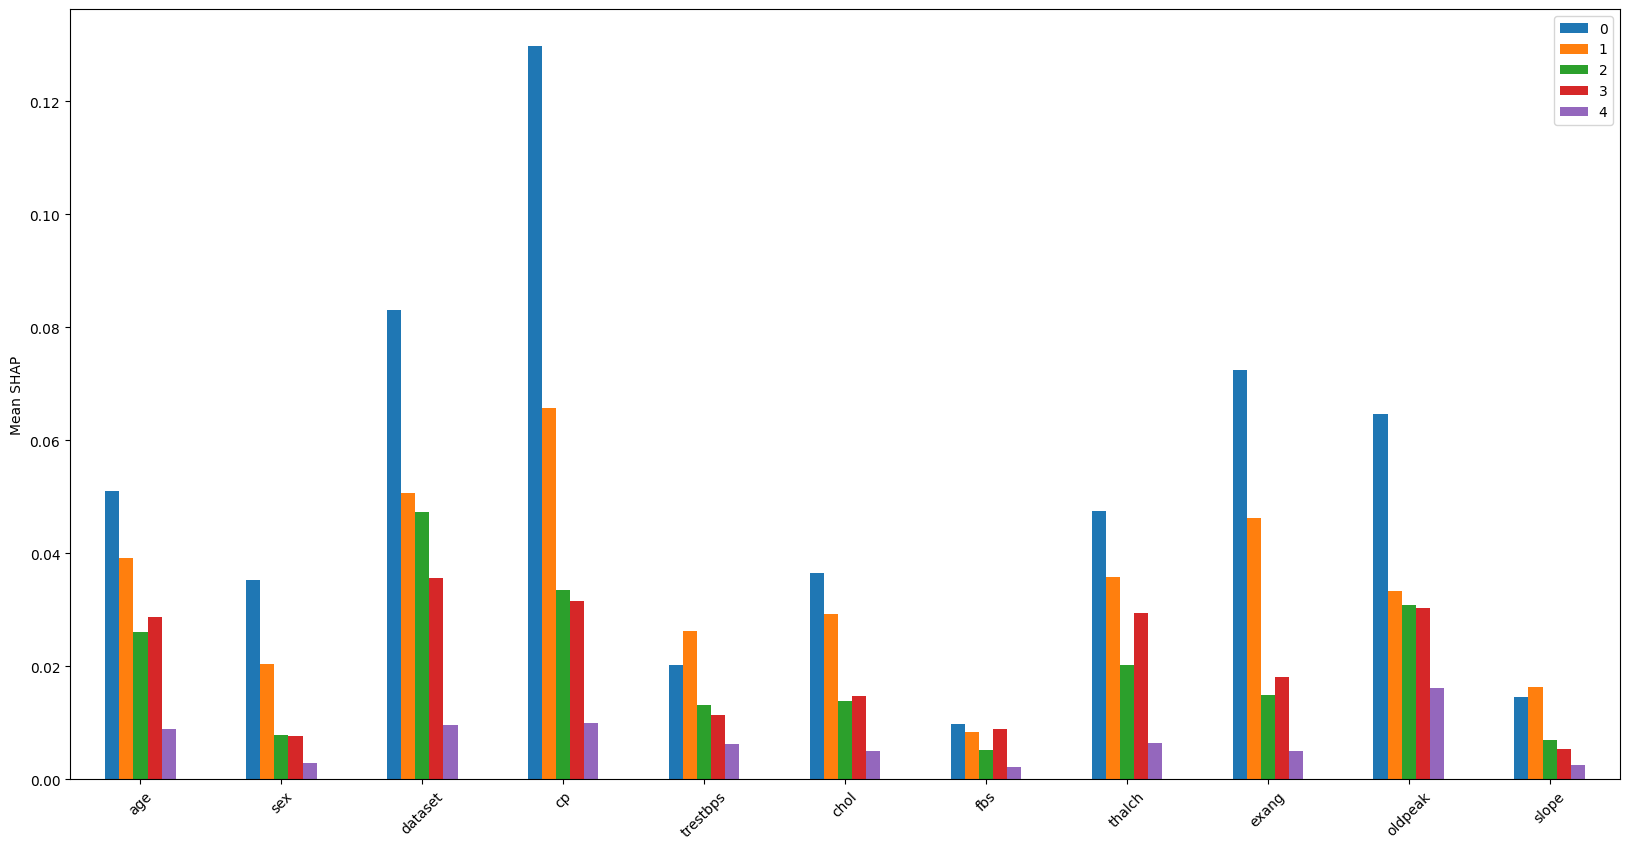
\includegraphics[width=0.85\linewidth]{rysunki/heart/shap_barchar_rf_heart.png}
    \caption{Przykładowy wykres słupkowy średnich wartości SHAP z podziałem na klasy [źródło własne]}
    \label{fig:shap_barchar_example}
\end{figure}

Skumulowane wartości bezwzględne SHAP, bez podziału na klasy, zebrane ze wszystkich próbek zbioru treningowego, tworzą średnie przedstawione na przykładowym wykresie słupkowym, zamieszczonym na Rys. \ref{fig:shap_absolutemeanplot_example}. Znajduje się na nim wyłącznie 10 elementów - 9 słupków najważniejszych cech oraz 1 przedstawiający połączenie reszty. Oś OY przedstawia cechy, a OX średnie wartości SHAP, których poszczególne wyniki zostały zamieszczone po~każdym z czerwonych pasków.

\begin{figure}[H]
    \centering
    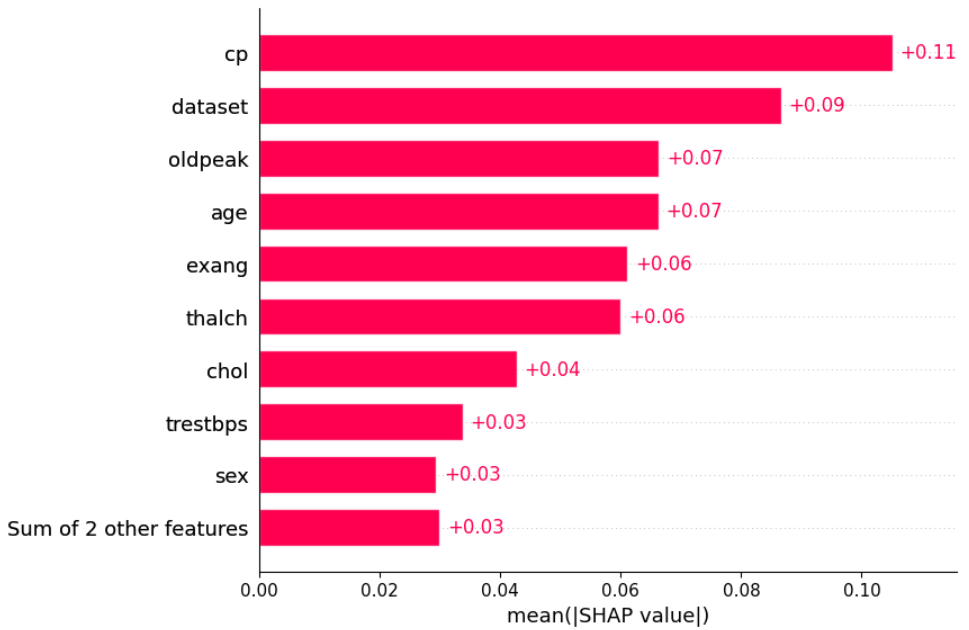
\includegraphics[width=0.70\linewidth]{rysunki/heart/shap_absolutemeanplot_rf_heart.png}
    \caption{Przykładowy wykres średnich obliczonych z bezwzględnych wartości SHAP [źródło własne]}
    \label{fig:shap_absolutemeanplot_example}
\end{figure}

Wykres typu ,,beeswarm'', przedstawiony na Rys. \ref{fig:shap_beeswarm_example}, prezentuje rozkład wartości cechy względem jej wpływu na predykcję modelu. Cechy są posortowane po ich wpływie na~wszystkie klasy. Jest to jedyna wizualizacja metody SHAP pokazująca, nie tylko wielkość, ale też, jakie znacznie ma badana cecha. Na osi OY zostało umieszczonych 9 najistotniejszych cech, reszta skumulowanO i przedstawionO na dole wykresu. OX oznacza wartości SHAP. Legenda znajdująca się po prawej stronie wizualizacji mówi o wielkości wartości cechy, gdzie niebieski kolor oznacza niską liczbę, a czerwony - wysoką. Wartości konkretnej cechy są przedstawione jako kropki w kolumnie jej odpowiadającej. Pionowa szara linia w~punkcie 0, to wartość średnia. Dla przykładu, zakładając, że sprawdzamy, czy osoba zarabia ponad 50 tys. PLN, to niebieskie kropki kolumny odpowiadającej wiekowi, umieszczone po lewej stronie od szarej linii (będącej tutaj średnią w wysokości badanej kwoty), oznaczałyby, iż młodzi ludzie najprawdopodobniej zarabiają mniej \cite{shap_beeswarmplot_explanation}. Jest on w pracy wykorzystywany jedynie w problemie klasyfikacji binarnej.

\begin{figure}[H]
    \centering
    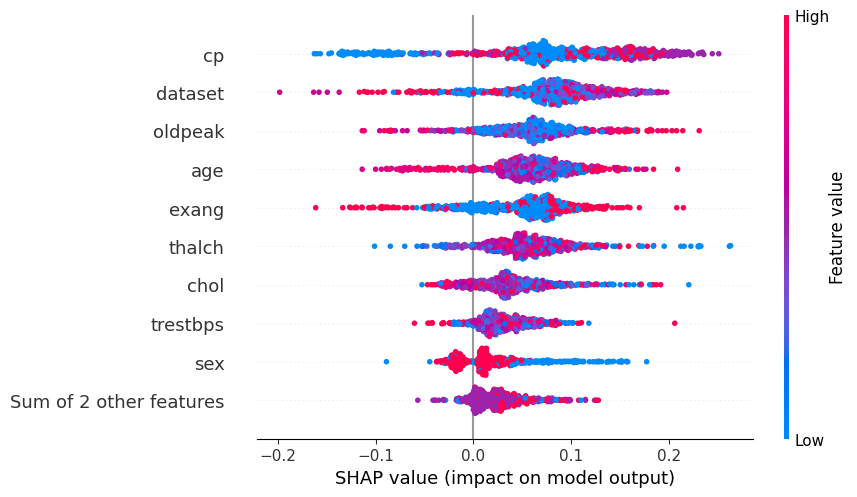
\includegraphics[width=0.85\linewidth]{rysunki/heart/shap_beeswarm_rf_heart.png}
    \caption{Przykładowy wykres typu ,,beeswarm'' wartości SHAP [źródło własne]}
    \label{fig:shap_beeswarm_example}
\end{figure}

Przykładowa wizualizacja, zaprezentowana na Rys. \ref{fig:shap_image_example}, przedstawia tłumaczenie przez metodę SHAP, próbki będącej obrazem. Wszystkie 3 fotografie przedstawiają obraz wejściowy. Na pierwszym z nich, nie dokonano żadnych zmian. Na drugim, zostało one wyszarzone oraz nałożono na nie maskę z wyjaśnieniem SHAP odpowiadającemu najbardziej prawdopodobnej predykcji. Na ostatnim, również zmniejszono widoczność próbki, a nałożona warstwa obrazuje wyjaśnienie dla drugiej najprawdopodobniejszej diagnozy, która w~klasyfikacji binarnej, jest klasą przeciwną do poprzedniej. Czerwone fragmenty przemawiają za danym wynikiem, niebieskie - się z nim nie zgadzają. Intensywność owych kolorów mówi, jak bardzo wpływowy jest dany obszar.

\begin{figure}[H]
    \centering
    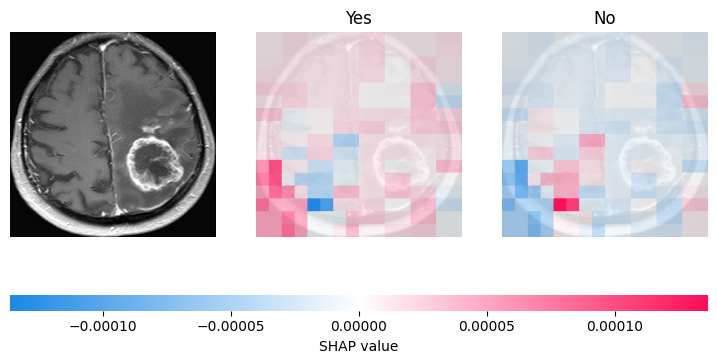
\includegraphics[width=0.8\linewidth]{rysunki/brain/shap_vgg16_1_brain.png}
    \caption{Przykładowe wyniki uzyskane po zbadaniu próbki za pomocą metody SHAP [źródło własne]}
    \label{fig:shap_image_example}
\end{figure}


\subsection{Permutation Feature Importance}
\textit{Permutation Feature Importance} (skrót PFI) \cite{molnar2025, pfi_documentation, permutation_importance_function}, które możemy tłumaczyć jako permutacyjna ważność cech, to bardzo prosta technika wyjaśniania modelu należąca do~niezależnych globalnych metod post-hoc. Jej działanie, przedstawione na Rys. \ref{fig:pfi_picture}, polega na~przepermutowaniu wartości cechy, a następnie zmierzeniu błędu predykcji. Jeżeli, po~owej zmianie, miara poprawności odpowiedzi naszego modelu zmaleje, to znaczy, że~badana cecha jest istotna. Dzieje się tak, ponieważ na niej opiera się przewidywanie, a jej przestawienie negatywnie wpłynie na jakość spodziewanego wyniku. Zaproponowany przez Fisher’a, Rudin’a i Dominici’ego w 2019 r. schemat, znakomicie obrazuje kroki tej techniki. Danymi wejściowymi są w nim: wytrenowany model predykcyjny oznaczony literą $m$, tabelaryczny zbiór cech (np. macierz) $X$, miara referencyjna (zazwyczaj błędu) $L$ i wartość docelowa (czyli ta, która jest poprawnym wynikiem przewidywania) $y$. Przebieg owego algorytmu:
\begin{enumerate}
    \item Oceń miarę referencyjną modelu oryginalnego, tu miarę błędu: 
    
    \begin{equation} \label{pfi_eqn}
    e_{origin}\ =\ \frac{1}{n_{test}}\ \sum_{i=1}^{n_{test}} L(y^{(i)},\ m(x^{(i)}))
    \end{equation}
    
    gdzie $n_{test}$, to wielkość zbioru testowego, na którym wyliczana jest szukana wartość.
    \item Dla każdej cechy należącej do zbioru $X$, tutaj określanej jako $j$ oraz powtórzenia $k$:
    
    \begin{enumerate}
        \item 	Stwórz nowy zbiór $X_{k,\ j}$ poprzez permutację wartości $j$ (np. losowe przetasowanie kolumny).
        \item 	Oceń miarę referencyjną zbioru $X_{k,\ j}$ na modelu $m$, analogicznie jak przy mierze oryginalnej (na tym samym zbiorze danych, ale ze zmodyfikowaną cechą $j$ - $x_{k,\ j}$ zamiast $x^{\left(i\right)}$)
        \item 	Oblicz istotność cechy ${FI}_j$ jako różnicę bądź iloraz miary referencyjnej zbioru zmienionego a oryginalnego. Poniższy wzór przedstawia różnicę:

        \begin{equation} \label{pfi_eqn2}
        {FI}_j=\ e_{k,\ j}-\ e_{origin}
        \end{equation}
    \end{enumerate}

    \item Posortuj wartości $FI$ (skrót od ang. \textit{Feature Importance}) malejąco.
\end{enumerate}

 \begin{figure}[H]
     \centering
     
\includegraphics[width=0.85\linewidth]{feature_premutation.png}
     \caption{Sposób działania metody PFI \cite{pfi_picture}}
     \label{fig:pfi_picture}
 \end{figure}

Metoda jest bardzo prosta, jednak posiada swoje ograniczenia. Jednym z nich jest możliwość zastosowania jedynie w przypadku danych tabelarycznych. Kolejnym - wymóg posiadania poprawnego wyniku przewidywań, to znaczy, że musimy użyć uczenia nadzorowanego, bo inaczej, nie będziemy w stanie obliczyć miary referencyjnej. Warto również zauważyć, iż ważność cechy jest tylko rankingiem, mówiącym jak bardzo zwiększy się miara straty, a nie to, czy zwiększenie jej poprawi prognozę. Dodatkowo, powinno się zwracać uwagę na~związki pomiędzy różnymi danymi, ponieważ, jeśli są one ze sobą silnie powiązane, to, przy permutacji którejś z nich mogą powstać fizycznie niemożliwe sytuacje.

Przykładowy wykres, znajdujący się na Rys. \ref{fig:pfi_boxplot_example}, obrazuje, jak permutacja cech wpływa na spadek dokładności według metody PFI. Oś OY prezentuje badane cechy, a OX zmniejszenie dokładności modelu. Na wizualizacji umieszczona została pionowa przerywana linia. Oznacza ona próg, od którego cecha jest brana pod uwagę i wynosi 0. Pudełka przedstawiają środkowe 50\% wartości, zielone pionowe kreski na nich - średnią, a~tak zwane ,,wąsy'' - wartości poza środkowymi 50\% \cite{khanacademy_boxplot}.     

\begin{figure}[H]
    \centering
    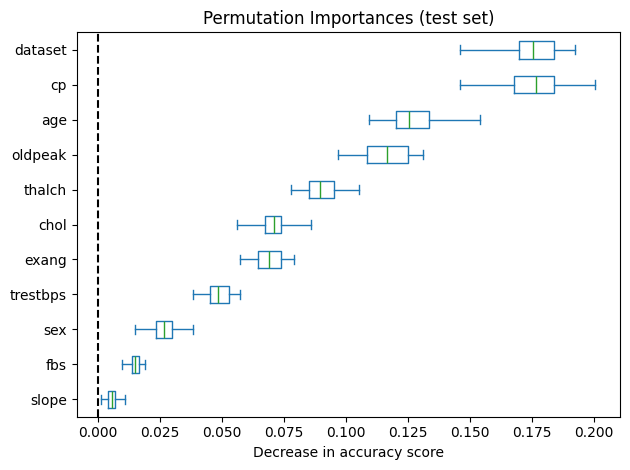
\includegraphics[width=0.65\linewidth]{rysunki/heart/pfi_rf_heart.png}
    \caption{Przykładowy wykres pudełkowy pokazujący wpływ cech na predykcję uzyskany po użyciu metody PFI [źródło własne]}
    \label{fig:pfi_boxplot_example}
\end{figure}


\subsection{Grad-CAM}
Grad-CAM (ang. \textit{Gradient-weighted Class Activation Mapping}) \cite{grad-cam_theory, grad-cam_theory2, ALI2023101805}, to specyficzna dla modelu metoda post-hoc służąca do analizy obrazów w konwolucyjnych sieciach neuronowych. Jej działanie, zobrazowane na Rys. \ref{fig:gradcam_picture}, polega na zaznaczeniu za pomocą mapy cieplnej (zwanej również mapą aktywacji klasy – ang. \textit{Class Activation Map (CAM)}) elementów badanego obiektu, które mają największy wpływ na jego klasyfikację. W tym celu wykorzystuje gradienty klas do wyznaczenia wag map w warstwach konwolucyjnych. 

Na początku podajemy dla naszej sieci obraz wejściowy i przeprowadzamy za jej pomocą klasyfikację. W taki sposób uzyskamy w całości uzupełnione mapy cech oraz logity, czyli wartości mówiące z jakim prawdopodobieństwem sklasyfikowano na obrazie cechę ze~zbioru możliwych klas nauczonych przez model. Następnie wybierany jest logit, niekoniecznie ten, który jest najprawdopodobniejszym rozwiązaniem. Teraz analiza ogranicza się do którejś z warstw splotowej sieci, w której znajdują się interesujące mapy cech. Zazwyczaj powinno się używać ostatniej z nich, ponieważ zawiera ona najistotniejsze części obrazu. 

Aby uzyskać pochodną logitu względem elementu mapy cech, czyli poszukiwany gradient, należy zastosować propagację wsteczną. Uzyskiwany jest w ten sposób wskaźnik pokazujący, jak zmiany w danej cząstce wpływają na wynik przewidywania. Dla każdego filtra wybranej wcześniej mapy konwolucyjnej wyznaczamy jego wagę poprzez średnią arytmetyczną gradientów jego elementów. Równanie to opisuje poniższy wzór:
\begin{equation} \label{grad_cam_filter_weight}
    a^c_k\ =\ \frac{1}{Z} \sum_{i} \sum_{j} \frac{\partial y^c}{\partial A^k_{ij}}  
\end{equation} 
gdzie $a^c_k$, to uzyskana waga filtra $k$, $Z$ oznacza liczbę gradientów, $i$ odpowiada szerokości na jakiej znajduje sie element, a $j$ wysokości; $\frac{\partial y^c}{\partial A^k_ij}$ jest gradientem, w którym $y^c$, to logit dla wskazanej wcześniej klasy decyzyjnej, natomiast $A^k_{ij}$ definiuje element. 

Aby uzyskać ważoną mapę cech, sumujemy mapy cech filtrów pomnożone przez odpowiadające im wagi.
Niektóre z jej elementów mogą posiadać ujemne wartości, wskazujące na~to, że dana instancja wpływała negatywnie na wybraną predykcję. Z tego powodu używamy funkcji aktywacji o nazwie ReLU, która zamienia wartości ujemne na zera. W~przedstawiony sposób uzyskujemy mapę cieplną o wielkości map cech w wybranej przez nas warstwie konwolucyjnej. W celu analizy należy zwiększyć jej rozmiar do tego, odpowiadającego obrazowi wejściowemu. Możemy tego dokonać wykorzystując \textit{upsampling} z technikami interpolacji. Proces ten polega na uzupełnieniu rozszerzanego obrazu poprzez wstawianie pikseli, pomiędzy te już istniejące, które mają jak najbardziej odpowiadać brakom \cite{interpolation_definition}. Grad-CAM można wykorzystać w tłumaczeniu różnego rodzaju sieci konwolucyjnych, jednak jego wyniki mogą być mało szczegółowe. 

 \begin{figure}[H]
     \centering
     
\includegraphics[width=0.85\linewidth]{grad_cam.png}
     \caption{Sposób działania metody Grad-CAM \cite{gradcam_picture}}
     \label{fig:gradcam_picture}
 \end{figure}

Na Rys. \ref{fig:gradcam_example} przedstawione zostały przykładowe wyniki metody Grad-CAM analizującej pojedynczą próbkę. Na lewym obrazku znajduje się mapa cieplna uzyskana za pomocą metody. Na prawym - zdjęcie wejściowe z nałożoną ów mapą. Im kolor jest jaśniejszy, tym zaznaczony obszar ma większy wpływ na wskazaną predykcję. Wynika z tego, że żółtym i limonkowym oznaczane są najważniejsze fragmenty, a odcieniami granatu i ciemnego fioletu - najmniej istotne.

\begin{figure}[H]
    \centering
    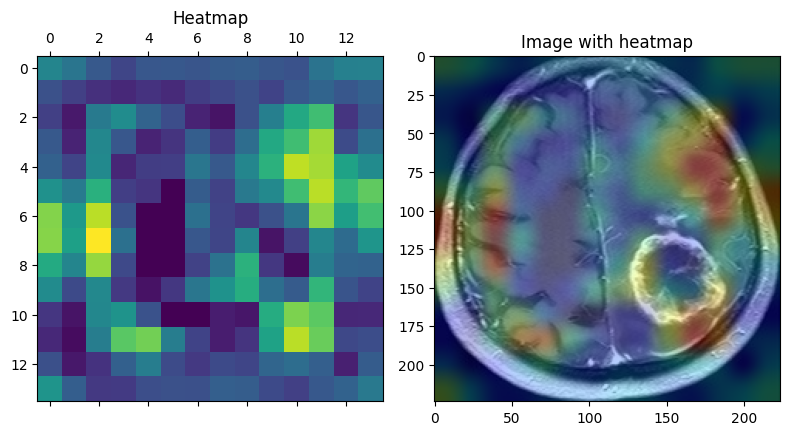
\includegraphics[width=0.55\linewidth]{rysunki/brain/gradcam_vgg16_1_brain.png}
    \caption{Przykładowe wyniki uzyskane po zbadaniu próbki za pomocą metody Grad-CAM [źródło własne]}
    \label{fig:gradcam_example}
\end{figure}


\subsection{Przegląd literatury}
Istnieje wiele prac naukowych wykorzystujących omówione metody. W przypadku danych tabelarycznych, w jednej z nich autorzy wykorzystują LIME i SHAP do tłumaczeń modeli LightBoost oraz XGBoost w zadaniu polegającym na przewidzeniu występowania choroby serca \cite{bioengineering11101016}. Wykazała ona, że metody są bardzo przydatne w zwiększaniu wydajności modeli poprzez aktywne uczenie polegające na informacji zwrotnej od eksperta w danej dziedzinie. 

Następne warte uwagi badania wykorzystują m.in. SHAP i PFI w tłumaczeniu algorytmu łączącego w sobie \textit{transfer learning}, \textit{autoencoder}'y i modele regresyjno-klasyfikacyjne w celu predykcji posiadania choroby Alzhaimera i MCI (ang. \textit{Mild Cognitive Impairment}) \cite{shap_pfi_research}. Wyniki badań wskazują, że metody mogą zostać wykorzystane równolegle - SHAP do globalnej oceny wpływów cech, a PFI do walidacji modelu. 

Inna praca wykorzystuje LIME i SHAP do wytłumaczenia decyzji regresji logistycznej i lasu losowego w zadaniu klasyfikacji osób chorych na cukrzycę \cite{10583856}. Konkluzją było wykorzystanie LIME do interpretacji konkretnych przypadków, a SHAP - całego zbioru. 

Kolejnym przykładem może być PFI użyty do poprawy jakości predykcji i kosztów obliczeń 5 modeli - drzew decyzyjnych, Ranger, Random Forest, Support Vector Machine, i k-najbliższych sąsiadów \cite{10900355}. Badanie potwierdziło, iż metoda rzeczywiście jest w stanie polepszyć osiągi - dokładności średnio o 77\%, a koszty obliczeń o 92\%.
 
Skupiając się na zbiorach złożonych z obrazów, należy wymienić pracę, gdzie wykorzystano LIME, SHAP i Grad-CAM w zadaniu wytłumaczenia klasyfikacji obrazów rezonansów magnetycznych mózgów na posiadające bądź nie zmiany nowotworowe \cite{NAZIR2024e38997}. Zostały one zastosowane na własnoręcznie zaprojektowanej konwolucyjnej sieci neuronowej. Z badań wynika, że SHAP poradził sobie najlepiej, oferując precyzyjne, spójne wyniki. LIME wypadł średnio - w niektórych przypadkach nie wskazywał szukanych zmian, pomimo ich występowania. Grad-CAM bardzo dobrze uwydatniał fragmenty mające pozytywne wpływy, ale również nie zawsze zaznaczał pożądane obszary.   

Kolejnym przykładem jest praca, w której LIME, SHAP oraz Grad-CAM zostały użyte do wytłumaczenia obrazu ptaka sklasyfikowanego przez ResNet50, a następnie poddane ocenie poprzez autorską metodę celem porównania efektywności i jakości ich wyników \cite{lime_shap_gradcam_research_images}. Uznano w niej, że Grad-CAM jest najlepszy pod względem czasu obliczeń, ale jego tłumaczenia są mało precyzyjne. Po przeanalizowaniu metod autorskimi sposobami, SHAP okazał się być najlepszym rozwiązaniem. 

XAI może być również wykorzystane do wyjaśnienia klasyfikacji obrazów zawierających znaki języka migowego. W jednej z prac w tym celu wykorzystano m. in. Grad-CAM i LIME do wytłumaczenia wyników modelu CNN wzorowanym na VGG-16 \cite{f98f8c14ef8e4c75a13839b615f87993}. Potwierdziły one poprawność wyników modelu. Autorzy zachęcali do zaimplementowania wszystkich badanych metod, argumentując swoją opinię ich ograniczeniami.

Wspomniane prace wskazują, jak przydatne i potrzebne są zaprezentowane metody. Pokazują ich słabe i mocne strony, niektóre typując jedno z XAI, jako szczególnie wyróżniające się spośród innych. Skupiają się one, jednak, na paru metodach i modelach oraz zbiorach danych należących do tej samej, zawężonej dziedziny. W tych badaniach oprócz 4 różnych metod, wykorzystanych zostało łącznie 6 odmiennych modeli, a także 4 zbiory, głównie danych medycznych, pozwalające na przeprowadzenie zadań klasyfikacji - 3 binarnej i jedno wieloklasowej. Dodatkowo zbiory dzielą się na 2 zestawy tabelaryczne i 2 obrazowe. Skutkuje to uzyskaniem obszernego porównania w niejednakowych problemach.


